\documentclass[a4paper, 11pt]{report}

\usepackage[utf8]{inputenc}
\usepackage[francais]{babel}
\usepackage{pdfpages}
\usepackage{graphicx}
\usepackage{parskip}

\setlength{\parindent}{0.7cm}

\title{Stage de 5ème année\\ \large Rapport intermédiare}
\author{Guillaume Delamare}
\date{\today}

\begin{document}
\maketitle

\section*{Remerciements}
Je tiens, tout d'abords, à remercier mon tuteur, Thomas Ledoux, pour m'avoir offert l'opportunité de travailler au sein de l'équipe ASCOLA. Je le remercie d'autant plus pour l'apport d'expérience et la richesse des situations dans lesquels il me fait travailler.

Je souhaite ensuite remercier Rémi Sharock, pour ça bonne humeur et son aide précieuse tout au long de mon travail, ainsi que, l'ensemble des membres de l'équipe ASCOLA et du département d'informatique de l'école des mines de nantes pour leur accueil, leur aide et leurs conseils.

Je remercie aussi mon encadrant, Benoit Parrain, pour l'aide et le suivi tout au long de cette exercice qu'est le stage de fin d'étude. Et pour finir je souhaite remercier Polytech Nantes, dans son ensemble, pour les trois années de formatin et d'encadrement dont j'ai pu profiter.

\newpage

\section*{Résumé}

\newpage

\tableofcontents



\chapter{Introduction}

\chapter{Contexte du stage}
\section{Présentation du lieu de stage}
Mon stage de cinquième année se déroule au sein de l’équipe ASCOLA du laboratoire LINA dans les locaux de l’école des Mines de Nantes.
\subsection{L'école des Mines de Nantes}
L’école des Mines de Nantes (EMN) est une école d’ingénieur française sous tutelle du ministère de l’industrie. l’école est rattaché à l’institut Mines-Télécom, au Groupe des écoles des mines et à la Conférence des grandes écoles.

Elle a été créée en 1990 sur le site de la chantrerie à Nantes et accueille 850 élèves ingénieurs en formation initiale. Le recrutement est effectué par concours après deux années de prépa. En 2011, l’EMN à décerné 250 diplôme d’ingénieur.

L’école est séparé en 5 départements de recherche :
\begin{itemize}
	\item Informatique
	\item Automatique et productique (DAP)
	\item Systèmes énergétiques et environnement (DSEE)
	\item Physique subatomique et technologies associées (Subatech)
	\item Sciences sociales et de gestion (DSSG)
\end{itemize}

\subsection{Léquipe ASCOLA}
L’équipe ASCOLA est installé au sein du département informatique de l’EMN. Elle se divise 
\section{Présentation du sujet de stage}
\subsection{Context}
Le stage se positionne dans les travaux GreenIT de l’équipe ASCOLA.
\subsection{Sujet}

\subsection{Objectifs}

\chapter{État de l'art}
\section{Introduction}
\subsection{Porté de l'éco-conception}
L’un des objectifs du Green IT est de réduire l’emprunte énergétique des systèmes d’informations (SI). Cette objectif a déjà été visé dans des travaux sur l'optimisation de la couche matérielle. Dans ce projet, nous souhaitons apporter un nouveau regard en étudiant l’impact du logiciel dans la consommation.

La réduction de l’emprunte énergétique peut être vu de plusieurs façons, qui sont autant d’objectifs intermédiaires pour notre projet :
\begin{itemize}
	\item Baisse de la consommation d’énergie
	\item Allongement de la durée de vie du matériel
	\item Augmentation de l’autonomie des appareils mobiles
\end{itemize}

L’éco-conception de logiciel consiste donc à travailler sur la composante logiciel afin d’améliorer ces critères.

\subsection{Qu'est ce qu'un code gourmand}
Répondre à cette question représente déjà une grande partie du travail de ce projet. Dans le cadre de ce projet nous souhaiterions parler de code gourmand au sens énergétique. Un parallèle est à faire avec la gourmandise d’un logiciel au sens efficacité. Cependant tout code efficace n’est pas forcement optimisé pour une faible consommation énergétique.

La définition d’un code gourmand est loin d’être trivial. En effet, la consommation d’un code est fortement lier à la tache pour la quelle il a été programmé. Un code servant à décoder un flux vidéo sera, énergétiquement, plus gourmand qu’un code servant à faire une addition. Cette exemple est extrême mais il montre bien qu’on peut difficilement comparer la gourmandise d’un code à un autre.

\subsection{Lien entre consommation énergétique et performance}

\section{Comment juger de l'éco-conception d'un logiciel}
\subsection{Annalyse du cycle de vie}
Expliquer que l’emprunte énergétique d’un logiciel n’est pas seulement du à la consommation lors du fonctionnement.
Étape de la vie d’un code
\begin{itemize}
	\item Conception
	\item Génération de Code (Méta modèle de code)
	\item Analyse statique
	\item Transformation de code (Compilation)
	\item Assemblage du programme (Linkage)
	\item Runtime (*PU)
\end{itemize}
Présentation du cycle de vie.
Aspect obsolescence matériel

\subsection{Mesure de la consommation d'un logiciel}
\subsubsection{Ptop}
pTop est un programme de collecte d’information sur l'exécution de processus sous linux.
\paragraph{Procédure d'installation}
\begin{itemize}
	\item récupérer les sources sur http://mist.cs.wayne.edu/ptop.html
	\item installation du nécessaire pour compiler les sources : build-essential libmysqlclient-devY libncurses-dev
	\item Installation de la base de données Mysql :
	\begin{itemize}
		\item création d’une base de donées ptop
		\item exécution du script db\_schema.sql
		\item remplacement du login et password pour accéder à la base de données dans le fichier database.c
	\end{itemize}
	\item Compilation :

\end{itemize}
\begin{verbatim}
	# make
	# chmod +x ptop
\end{verbatim}

\paragraph{Exécution}
Lancer le programme au moyen de la commande :

\begin{verbatim}
# ./ptop
\end{verbatim}

Le programme va s'initialiser et enregistrer les mesures dans les bases de données. Il faut ensuite interrompre les mesures au moyen du signal SIGINT.

\paragraph{Données de sortie}
Il n’existe pas, à ma connaissance, de documentation précise sur les données de sortie du programme pTop. Je répertorie donc ici des informations issus de mes déductions. Le programme stock les données dans une base de données Mysql nommé ptop. Elle est composé de quatre tables :
\begin{itemize}
	\item device\_energy
	\item process\_energy
	\item process\_info
	\item sys\_info
\end{itemize}

Seul les deux dernières tables sont remplis par le programme (à cause soit d’un bug, soit d’une version non finit du programme).

\subsubsection{Energy Checker}
Le projet Energy Checker développé par Intel, est un ensemble d’outil destiné à faciliter la remonté et l’affichage des mesures faites sur la consommation d’un programme. Il se compose principalement de l’API energy checker qui permet d’utiliser les mécanisme de remonté d’imformation (PL - Productivity Link)

\subsubsection{ClassMexer}
ClassMexer est un API java permettant d’estimer la taille en mémoire d’un objet java. On peut télécharger cet API sous la forme d’un fichier JAR à cette adresse : http://www.javamex.com/classmexer/

ClassMexer est un Instrumentation agent comme spécifié dans le pattern Instrument. Cela implique de travailler avec, au minimum, la version 5 de java.

\paragraph{procédure d'installation}
\begin{itemize}
	\item Télécharger l’API
	\item Importer le fichier JAR dans le projet.
	\item Insérer des appels sur l’objet que l’on souhaite mesurer. Par exemple :
\begin{verbatim}
public class Main {
	public static void main(String[] args) {
		String str = "Hello world !";
		
		long noBytes = MemoryUtil.deepMemoryUsageOf(str);
		
		System.out.println(noBytes);
	}
}
\end{verbatim}
	\item Exécuter le programme avec l’option -javaagent:<fichier JAR>
\end{itemize}

\subsubsection{JouleMeter}
Joulemeter est un outil développé par microsoft et qui sert à mesurer la consomation d’énergie sur un ordinateur. Il ne fonctionne que sous Windows 7.

\paragraph{Procédure d'installation}
\begin{itemize}
	\item Télécharger le logiciel sur ce site : Joulemeter
	\item Exécuter le programme.
\end{itemize}

\paragraph{Fonctionnement}
Joulemeter est un logiciel de mesure qui se base sur un modèle de consommation. la première étape est donc de générer ce modèle. Deux méthodes existe.

La première n’est utilisable que sur un ordinateur portable muni d’une batterie. Il suffit de débrancher l’alimentation et de lancer la calibration (15 min sans utiliser le PC). Avant de lancer la calibration, il faut faire attention à arrêter toutes les application affin que le logiciel puisse déterminer une consommation minimum en mode Idle.

Le deuxième mode nécessite un Wattmètre WattsUp pour générer le modèle. Il suffit de le brancher en USB, de couper toutes les application possible et de lancer la calibration (3 min sans utiliser le PC).

\subsubsection{PowerAPI}
Pas disponible (donc pas testé)
Sujet de recherche
Développé en ce moment par l’équipe ADAM à l’université de Lilles.
fonctionne actuellement pour la consommations CPU.
Se base sur l’outil linux cpufrequtils
étudie la fréquence utilisé par le CPU
détermine une consommation global du CPU grâce au donnée constructeur (table de correspondance fréquence/Volt).
détermine la consommation d’un processus grace à son taux d’utilisation du CPU.
\subsection{Métriques}
\begin{itemize}
	\item PUE (Power Usage Effectiveness)
	\item ERE (Energy Reuse Effectiveness) (ref)
	\item CUE (Carbon Usage Effectiveness)
\end{itemize}
L’indice PUE met en valeur la perte énergétique des équipements. Il ne prend pas en compte la valorisation de ces pertes.
L’indice ERE essai de rattraper les faiblesses du PUE en prenant en compte la revalorisation.
L’indice CUE permet de valoriser le type d’énergie utilisé.

\section{Bonnes pratiques et patrons de conception}
\subsection{Modularité}
Décrire les différence entre programme Monolithique et programme modulaire
	Liens avec les OS (Monolithique Vs Micro noyau)
	Linux serait monolythique au sens OS mais modulaire au sens logiciel ?

POO = modulaire ?
	Si oui qu’est ce qu’est OSGi
	Début de réponse : OSGi = approche Objet au niveau architecture logiciel

Question de la compatibilité inter-langage des modules. Comment rendre modulaire un programme au point qu’il fonctionne de la même façon quelque soit les langage d’origine de ses module.

Qu’est ce qu’un module en théorie ?
\begin{figure}
	\begin{center}
		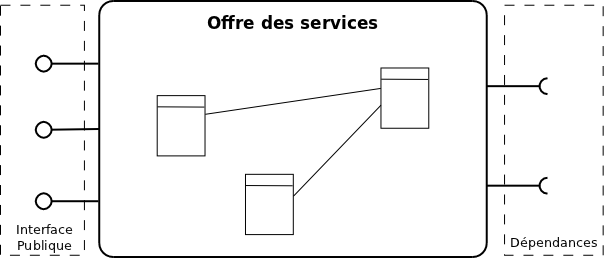
\includegraphics[width=300px]{../../Figures/Bibliographie/modular.eps}
		\caption{Repsésentation d'un module}
	\end{center}
\end{figure}

\begin{itemize}
	\item Cohérence des services offert dans un module. -> éviter de faire une boite à outils pour tout faire.
	\item Offre ses services au travers d’une interface public.
	\item Privilégié l’utilisation/dépendance à d’autre module plutôt que l’encapsulation ou la réécriture au sein du module.
	\item Un module qui fournis un service peut être remplacé par un autre module qui fournis le même service.
\end{itemize}
\subsection{OSGi}
modularité de code = activation ou désactivation de module. Cela libère de la ressource mais implique certainement une contrepartie : par exemple des accès disque multiplié pour activer un module.

OSGI est une spécification, élaboré par l’OSGi Alliance (http://www.osgi.org), qui à pour but de décrire un framework pour rendre les applications Java modulaire. Différentes implémentation de ce framework ont été développé à partir de cette spécification. Les plus connu sont Equinox développé par l’équipe du projet eclipse, Felix issu du projet universitaire Oscar et maintenu par apache ou encore Knopflerfish élaboré par MakeWave.
\section{Conclusion}

\chapter{Propositions}

\chapter{Conclusion}

\appendix

\chapter{Sujet de stage}
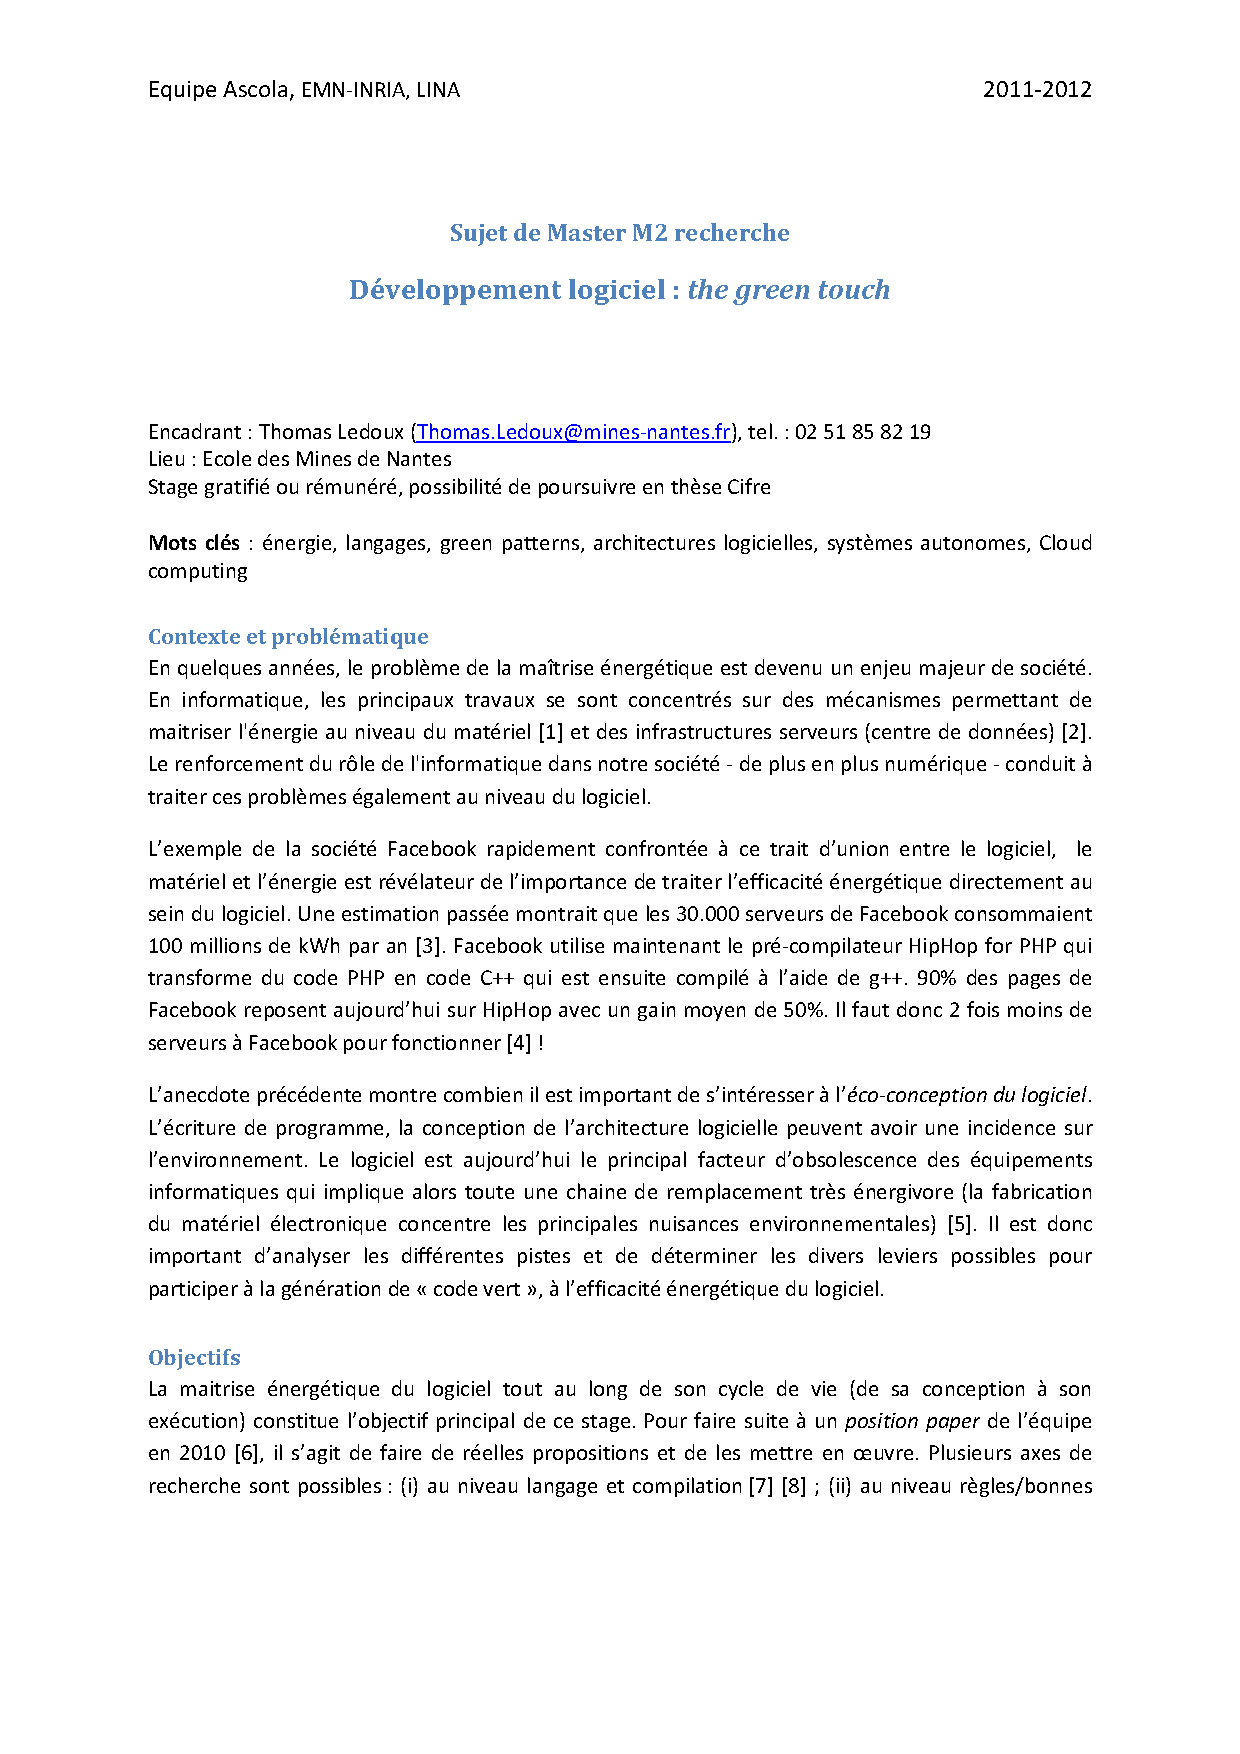
\includepdf[pages=-]{../../Documents/Sujet_Master_EcoConceptionGL.pdf}

\chapter{Projets similaire}

\listoffigures{}
\listoftables{}

\end{document}
